\documentclass{acm_proc_article-sp}% {article}% TODO: twosided

%%%%% BASIC PACKAGES %%%%%%%%%%%%%%%%%%
% Support for Danish characters UTF-8
\usepackage{ucs}
\usepackage[utf8x]{inputenc}

% English bibliography
\usepackage[english]{babel}

% Coloring of text and tables
\usepackage{color}
\usepackage{colortbl}


% Framed boxes
\usepackage{framed}

% Allow for custom floats
\usepackage{float}

% Landscape environment
\usepackage{lscape}

% inline lists
\usepackage{paralist}

%Compact versions of bullet lists: itemize*, enumerate* and description* 
\usepackage{mdwlist}

% MATHEMATICS
%\usepackage{amsthm}			% AMS theorem package
\usepackage{amsfonts}
\usepackage{amsmath}		% AMS math symbols
\usepackage{amssymb}		% More symbols!
\usepackage{mathtools}		% Even more symbols!
\usepackage{latexsym}		% Holy shit I can't believe there are still more symbols!
\usepackage{stmaryrd}		% Symbols! When will it end?
\usepackage{textcomp}		% The unholy God of symbols has spoken. We need more symbols
\usepackage{gensymb}

% ALGORITHMS
%\usepackage{algorithmic}
\usepackage[ruled]{algorithm}
\usepackage{algpseudocode}
%Algorithmic should use "Input:" and "Output:" instead of "require:" and "ensure:"
\algrenewcommand{\algorithmicrequire}{\textbf{Input:}}
\algrenewcommand{\algorithmicensure}{\textbf{Output:}}

%Multiline comments etc..
\usepackage{verbatim} 

%Figures and tabels
%\usepackage[pdftex]{graphicx}	% JPEG, PNG
\usepackage{wrapfig}			% Stuff for wrap figs
%\usepackage{subfig}				% insert several subfigures in a figure
\usepackage{flafter}			% prevents floats from appearing before their definiton
\usepackage{sidecap}			% Allows text next to image
\usepackage{array}				% Used with tables - give the ability to align text to center or bottom of cell.
\usepackage{multirow}			% Used to create multi column and multi row spanning cells.
\usepackage{multicol}			% Same as multirow, but for columns. (This package may be redundant)
\usepackage{longtable}			% Tables split over several pages
%\usepackage{slashbox}			% Slashed cells, eg. boxes that are split diagonally

%Path for images, images are in image/, compiled images are in bin/images/
\graphicspath{{bin/images/}}

%Allow LaTeX to accept images with dot in the filename
\usepackage{grffile}

\usepackage{pgfplots}
\pgfplotsset{width=6cm, height=5cm}

%For ensuring space after commands
\usepackage{xspace}

% Conditionals nice
\usepackage{ifthen}

% Really, really slack formatting
% This relaxes what is considered "bad" formatting,
% and should suppress warnings ala "underfull \hbox" and the like
\tolerance=10000            % Knuth-infinite
\hbadness=10000
\emergencystretch=1.5em     % EMERGENCY STETCH
\hfuzz 10000pt
\widowpenalty=10000
\vfuzz \hfuzz
\raggedbottom

%See http://www.eng.cam.ac.uk/help/tpl/textprocessing/squeeze.html
\setlength{\intextsep}{1.5ex}
%\setlength{\floatsep}{1ex}
%\setlength{\textfloatsep}{1ex}
%\addtolength{\intextsep}{-4ex}
%\addtolength{\floatsep}{-4ex}
%\addtolength{\textfloatsep}{-4ex}

% HYPERLINKS
% Enables www-urls:
\usepackage{url}
% Enables hyperlinks:
\usepackage[pdftex]{hyperref}
\hypersetup{
    pdftoolbar 		= true,        					% show Acrobat’s toolbar?
    pdfmenubar 		= true,        					% show Acrobat’s menu?
    pdffitwindow 	= true,      					% page fit to window when opened
    pdftitle 		= {Characterising Eco driving with GPS and CANbus data},    	% title
    pdfauthor 		= {Karsten Jakobsen and Sabrine Conny Hj\oe llund Mouritsen}, 
    pdfsubject 		= {Computer Science},   		% subject of the document
    pdfcreator 		= {LaTeX},   					% creator of the document
    pdfproducer 	= {PdfLaTex}, 					% producer of the document
    pdfkeywords 	= {Computer Science}, 			% list of keywords
    pdfnewwindow 	= true,      					% links in new window
    colorlinks 		= true,       					% false: boxed links; true: colored links
    linkcolor 		= black,          				% color of internal links
    citecolor 		= black,        				% color of links to bibliography
    filecolor 		= black,      					% color of file links
    urlcolor 		= black           				% color of external links
}

%%%%% CUSTOM MACROS %%%%%%%%%%%%%%%%%%%
\newtheorem{definition}{Definition}

\newcommand{\heltal}{\ensuremath{\mathbb{N}}\xspace}


\begin{document}

\title{Characterising Eco driving with GPS and CANbus data}

\numberofauthors{2}
\author{
% Separate each 3 authors with an 'and'
% 1st. author
\alignauthor
Karsten Jakobsen\\
       \affaddr{Institute of Computer Science}\\
       \affaddr{Aalborg University}\\
       \affaddr{Denmark}\\
       \email{karstenjjakobsen@gmail.com}
% 2nd. author
\alignauthor 
Sabrine C. H. Mouritsen\\
       \affaddr{Institute of Computer Science}\\
       \affaddr{Aalborg University}\\
       \affaddr{Denmark}\\
       \email{sabrinechm@gmail.com}
}

\date{1th of July 2013}
\maketitle

%%%%%%%%%% DO NOT EDIT BELOW, THIS WILL BE AUTO GENERATED %%%%%%%%%%
%\input{src/Abstract.tex}
%\keywords{}
\section{Introduction}

Reducing fuel consumption and greenhouse gas emissions is important.

What is Eco-driving? \cite{EcodrivingAdvice}
\begin{itemize}
\item Shift up as soon as possible
\item Maintain a steady speed
\item Anticipate traffic flow
\item Decelerate smoothly
\item Avoid idling
\item Avoid pressing the accelerator when switching on engine
\item Minimise additional weight
\item Minimise air resistance
\item Maintain correct tyre pressures
\item Avoid fuel consuming accessories, e.g. air-conditioning
\item Use fuel saving in-car devices as revolution counter and cruise control
\end{itemize}



We aim to identify which factors, available through GPS and CANbus data, has an influence on
fuel consumption and how one explains the difference in the fuel consumption of different
vehicles of the same type?

Contributions
\section{Related Work}

EcoMark \cite{EcoMark}, can eleven models for fuel consumption be used to do eco driving and/or eco routing?

GreenGPS \cite{GreenGPS}, how to find fuel efficient routes.

INTEGRATION model framework \cite{IMF}, quantifying environmental impact.

\cite{EvalEcoDriving}, How does instantanious fuel economy feedback affect driving behaviour?

\cite{Barth}, Real time dynamic advice on speed in order to save fuel 

\cite{Beusen}, Long-term effect of Eco-driving cources.
\section{Data Description}
<<<<<<< HEAD

\begin{table}[htb]
\begin{tabular}{|l|l|l|l|}\hline
Name & Data type & Source & Description\\\hline
\var{vehicleid} & integer & ID & Unique identifier for vehicles\\\hline
\var{timestamp} & timestamp & GPS & Date and time of the record\\\hline
\var{longitude} & float & GPS & Longitude coordinate of the vehicle\\\hline
\var{latitude} & float & GPS & Latitude coordinate of the vehicle\\\hline
\var{speed} & float & GPS & Driving speed in km/h\\\hline
\var{direction} & integer & GPS & Direction of the vehicle in degrees. North (0), east(90), south(180) and west(270)\\\hline
\var{satellites} & integer & GPS & Number of visible satellites\\\hline
\var{rpm} & integer & CANBus & The engines rounds per minute\\\hline
\var{kmcounter} & float & CANBus & Mileage record\\\hline
\var{temperature} & float & CANBus & Temperature of the engine in degrees Celsius\\\hline
\var{throttlepos} & float & CANBus & Position of the throttle. No data available\\\hline
\var{fuellevel} & float & CANBus & Fuel level in the tank where 100 is full tank.\\\hline
\var{totalconsumed} & float & CANBus & Total amount of fuel consumed by the vehicle in liters\\\hline
\var{actualconsumed} & float & CANBus & Instantaneous amount of fuel consumption in liters. Undependable\\\hline
\var{actual\_km\_l} & float & CANBus & Instantaneous km/l. Undependable\\\hline
\var{acceleration} & float & CANBus & Acceleration ???\\\hline %TODO: What is this
\var{make} & integer & Haulier &The make of the vehicle. No data available\\\hline
\var{model} & integer & Haulier &The model of the vehicle. No data available\\\hline
\var{capacity} & float & Haulier & Number of possible passengers. No data available\\\hline
\var{weight} & float & Haulier & The weight of the vehicle. No data available\\\hline
=======
\\
\begin{table}[htb]
\begin{tabular}{|l|l|l|l|}\hline
Name & Data type & Source & Description\\\hline
vehicleid & integer & ID & Unique identifier for vehicles\\\hline
timestamp & timestamp & GPS & Date and time of the record\\\hline
longitude & float & GPS & Longitude coordinate of the vehicle\\\hline
latitude & float & GPS & Latitude coordinate of the vehicle\\\hline
speed & float & GPS & Driving speed in km/h\\\hline
direction & integer & GPS & Direction of the vehicle in degrees. North (0), east(90), south(180) and west(270)\\\hline
satellites & integer & GPS & Number of visible satellites\\\hline
rpm & integer & CANBus & The engines rounds per minute\\\hline
kmcounter & float & CANBus & Mileage record\\\hline
temperature & float & CANBus & Temperature of the engine in degrees Celsius\\\hline
fuellevel& float & CANBus & Fuel level in the tank where 100 is full tank.\\\hline
throttlepos & float & CANBus & Position of the throttle. No data available\\\hline
totalconsumed & float & CANBus & Total amount of fuel consumed by the vehicle in liters\\\hline
actualconsumed & float & CANBus & Instantaneous amount of fuel consumption in liters. Undependable\\\hline
actual\_km\_l & float & CANBus & Instantaneous km/l. Undependable\\\hline
acceleration & float & CANBus & Acceleration ???\\\hline %TODO: What is this
make & integer & Haulier &The make of the vehicle. No data available\\\hline
model & integer & Haulier &The model of the vehicle. No data available\\\hline
capacity & float & Haulier & Number of possible passengers. No data available\\\hline
weight & float & Haulier & The weight of the vehicle. No data available\\\hline
>>>>>>> 674bfc2e2dc120153c3619195e276d820b5c71b6
\end{tabular}
\caption{GPS and CANBus data types}\label{tb:dataDescription}
\end{table}
\clearpage

A number of data sources can be used to gather data.
GPS data can easily be collected from any vehicle equiped with a GPS system, through which for example a timestamp, longitude, latitude and speed are available.
CANBus data provides information about the state of the vehicle.  %TODO: Reformulate
Retriving CANBus data is not as easy as GPS data, and little data is therefore avialable. 
CANBus data is for example the engines rounds per minute, fuel consumption and temperature. 
The hauliers may also provide additional information such as vehicle model, capacity and weight. 

Table~\ref{tb:dataDescription} lists the data columns in the provided data set.
The data set contains 10,224,846 records collected from 6 minibusses. 
All vehicles are assumed to be compareable.%TODO
<<<<<<< HEAD

Of the four columns for fuel comsumption, \var{totalconsumed} is the most accurate measure.
The instantaneous values, i.e. \var{actualconsumed} and \var{actual\_km\_l}, is said to be undependable by the data provider and should not be used. 
\var{fuellevel} is fuel level in the tank in percentage (100 \% is full and 0 \% is empty) and \var{totalconsumed} is the amount of fuel consumed.
\var{totalconsumed} does only have a granularity of half a liter, which means it can only be used at an agreegated level of at least a trip in order to get usable results.

Non of the data provided by the haulier is available.
=======
Instantaneous fuel consumption is undependable and should not be used and non of the data provided by the haulier is available.
totalconsumed is the most accurate measure for fuel consumption, however, it only has a granularity of half a liter. Therefore, it can only be used at an agreegated level of at least a trip.
>>>>>>> 674bfc2e2dc120153c3619195e276d820b5c71b6

\section{Data Grouping}
Only grouping the data on vehicles will give too few and too diverse groups of which it will be difficult to make usable conclusions. 
The data therefore needs to be grouped into smaller units.
In the following we will use two different grouping strategies, periods and trips, explained in the sections below.
Figure~\ref{fig:groupings} shows the two concepts.
The top lines indicate three trips where the ``gaps" represent time between two trips.
A trip can thereafter contain smaller periods indicated by the boxes below.
A period is a stretch of time where some property holds, e.g. the vehicle drives at the same speed or the vehicle is idling.

\begin{figure}[htb]
\centering
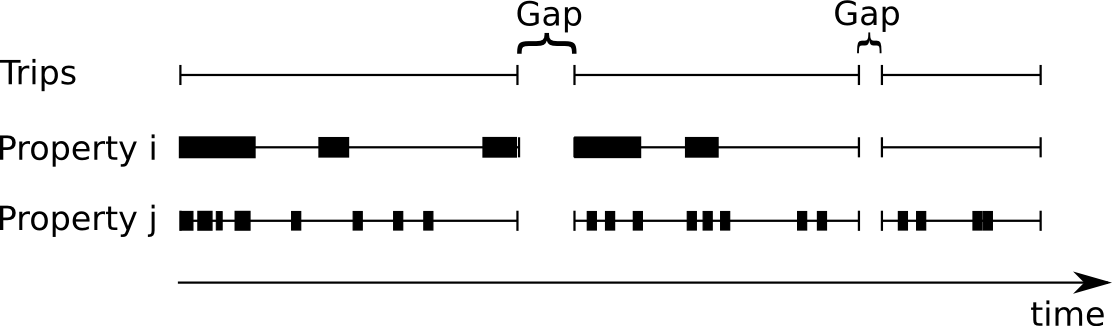
\includegraphics[width=0.45\textwidth]{../images/groupings.png}
\caption{Example of periods and trips}
\label{fig:groupings}
\end{figure}

\subsection{Trips}\label{sec:trips} 
This temporal and sometimes spatial grouping looks primarily on the time difference between trips, the length of the trip and sometimes the location of the vehicle.
The data set is split into trips by annotating each record with a trip identifier, \tid{\rec{}}.
A trip, \trip{} is defined as a consecutive sequence of at least 30 records with the same vehicle identifier where the engine is turned on and any two consecutive records are within 120 seconds.
\begin{align} %TODO: I still do not like this one
\timestamp{\rec{j+1}}-\timestamp{\rec{j}}&< 120\nonumber\\
|\trip{}|&\geq 30\nonumber\\
\tid{\rec{j}}=\tid{\rec{j+1}}&=\tid{\trip{}}\nonumber\\
\vid{\rec{j}}=\vid{\rec{j+1}}\nonumber
\end{align}
where $j$ ranges over the records in the trip.

Idle time, i.e. when the engine is running but the vehicle is not moving (see Section~\ref{sec:idle}), is an important factor for fuel consumption, and we therefore need to ensure that these records are included in the trips. 
A trip is hence defined from when the engine of the vehicles engine is running, that is when $\rpm{\rec{}}> 0$.
In order not to split a trip into two just because the engine stalls, we say that a trips ends when the time cap between two consecutive records is too large.
Figure~\ref{fig:TimeTrips} shows the number of trips when varing the time gap from 5 seconds between two trips to 200 seconds.
We see that the curve flattens around 120 seconds and we choose this as the gap.
Short trips with few records will not give a usable idea of which factors influence fuel consumption.
Figure~\ref{fig:LengthTrips} show the number of trips varying the minimum number of records in a trip.
The curve flattens around 30 records, which in most cases will correspond with 30 seconds. 
A similar test using time as the minimum requirement on trips show no clear result. 
\begin{figure}[htb]
\centering
\includegraphics[width=0.45\textwidth]{../src/d_images/TimeTrips.png}
\caption{Number of trips at different timeframes}
\label{fig:TimeTrips}
\end{figure}
\begin{figure}[htb]
\centering
\includegraphics[width=0.45\textwidth]{../src/d_images/TripsLength.png}
\caption{Number of trips at different lengths}
\label{fig:LengthTrips}
\end{figure}

\subsection{Periods}\label{sec:periods}%TODO: Other name?
It will some times be more interesting to look at records with a similar propery than looking solely at trips.
Let a period be a sequence of consecutive records within a trip with some similar property.
The example in Table~\ref{tb:periods} shows two period groupings on a small sample set.
The property of period X is that the speed is exactly the same as that of the previouse record.
The sample set hence contains 2 periods with this property.
The propery of period Y is that the vehicle is accelerating which results in two different periods.
Let $\timelength{p}$ be the length of period, $p$ in seconds. %TODO: Do we use this?

\begin{table}
\centering
\begin{tabular}{|c|c|c|c|c|}\hline
record id & speed & tid & Period X & Period Y\\\hline
\rec{1} & 59 & 0 &   & a \\\hline
\rec{2} & 60 & 1 & 1 & a\\\hline
\rec{3} & 60 & 1 & 1 &  \\\hline
\rec{4} & 60 & 1 & 1 &  \\\hline
\rec{5} & 63 & 1 &   & b\\\hline
\rec{6} & 64 & 1 &   & b\\\hline
\rec{7} & 67 & 1 & 2 & b\\\hline
\rec{8} & 67 & 1 & 2 &  \\\hline
\rec{9} & 67 & 2 &   &  \\\hline
\end{tabular}
\caption{Example of period grouping}\label{tb:periods}
\end{table}



\section{Kilometers per liter fuel}

How many kilometers(km) per liter fuel (km/l) a vehicle drives will indicate how fuel efficient the vehicle is.
The main goal of a vehicle is transportation and hence, the more kilometers one can drive per liter fuel, the cheaper it is.

Let $\kml{t}$ be the total number of km driven in trip $t$ devided by the total fuel consumption of trip $t$, and let $\kml{v}$ be the average of $\kml{t}$ for all trips that vehicle $v$ has driven.

Figure~\ref{fig:kmlTrips} plots all $\kml{t}$ with trips on the x-axis, $\kml{t}$ on the y-axis and a plot symbol for each vehicle.
We see that the majority of the trips have a $\kml{t}$ between 5 and 10 km/l, but also that many trips have a near zero value.
The latter is because they do not drive anywhere.
This is very consistent with what can be expected from minibusses.

All trips are devided into classes based on their $\kml{t}$, such that we later can classify the different factors. %TODO: Uklart
All trips with $\kml{t}\leq4$ are in the \fuelLow class. These trips have an distinctively low km/l and lie out side of the normal range. 
The remaining trips are grouped in two to classes, \fuelMedium and \fuelHigh in order to distinquish the best from the rest.
\fuelMedium contains trips with $4 < \kml{t} < 8$ and \fuelHigh contains trips with $\kml{t}\geq8$.
Had we only used two classes, e.g. 0 to 4 and above 4, will allow us to identify very bad trips but not average versus good. 
One could also have a class containing trips with more than 10 km/l but only 94 trips will be in this class. %CHECK
\begin{figure}[htb]
\centering
%\includegraphics[width=0.5\textwidth]{../src/images/kmlTrips.png}
\caption{km/l for all trips}
\label{fig:kmlTrips}
\end{figure}


\section{Avoid Idling}

Avoid idling or minimising idle time is a factor in eco-driving, as fuel is still consumed when the engine is running even though the vehicle is not moving.
The driver is hence consuming unneccesary fuel when idling.

A vehicle is idling when the engines rounds per minute (RPM) is above zero while the speed is zero for at least X consecutive recordings. %CHECK
Let $\vrpm$ and $\vspeed$ be the RPM and speed of vehicle $v$ at time $t$, then a vehicle is ideling when
\[\mbox{\textbf{for }} i, \dots ,t, \dots, i+X \mbox{: }\vrpm> 0 \wedge \vspeed=0 \]
A vehicle must be in idling at least $X$ seconds in order to eliminate involuntary idle times at for example traffic lights or due to small disturbances is the traffic flow.
Figure~\ref{fig:idleDuration} plots a graph of the number of records in which a vehicle is idling at different minimum durations. 

\begin{figure}[htb]
\centering
\includegraphics[width=0.5\textwidth]{../src/images/idleDuration.png}
\caption{Minimum idle duration}
\label{fig:idleDuration}
\end{figure}

Figure~\ref{fig:idleTime} plots the km/l for all trips as a function of how many seconds the vehicle has been idling.
The size of the plot indicates the amount of fuel used in the trip and the color signals what class it has been asigned to.
TODO: analyse
\begin{figure}[htb]
\centering
\includegraphics[width=0.5\textwidth]{../src/images/idleTime.png}
\caption{Idle time}
\label{fig:idleTime}
\end{figure}

It might give a more fair result, if the numbers from Figure~\ref{fig:idleTime} are normalised such that the x-axis plots how many percent of the records are an idle state compared to the number of records in the trip.
Figure~\ref{fig:idlePercent} plots the km/l for all trips as a function of how many percent of the trip the vehicle has been idling.
The size of the plot indicates the amount of fuel used in the trip and the color signals what class it has been asigned to.
TODO: analyse
\begin{figure}[htb]
\centering
\includegraphics[width=0.5\textwidth]{../src/images/idlePercent.png}
\caption{Idle percent}
\label{fig:idlePercent}
\end{figure}

Figure~\ref{fig:idleClassPercent} abstracts away the actual km/l and only plots the class distibution as a function of he idle percent. 
The purple line indicates how many trips have this idle percentage. 
The graph is cut off at 60 \% because of too little data.
It is evident that the majority of the trips in the \fuelHigh class avoids idling. 
TODO: analyse

\begin{figure}[htb]
\centering
\includegraphics[width=0.5\textwidth]{../src/images/idle2.png}
\caption{Class distribution }
\label{fig:idleClassPercent}
\end{figure}

\begin{figure}[htb]
\centering
\includegraphics[width=0.5\textwidth]{../src/images/idle3.png}
\caption{Class distribution}
\label{fig:idleClassTime}
\end{figure}


\section{Defintions}
\subsection{Trips}
The data set is split into trips by annotating each record with a trip identifier, \tid.
A trip is defined as a collection of consecutive records with the same vehicle identifier, \vid.
Idle time, i.e. when the engine is running but the vehicle is not moving, is persumed to be an important factor for fuel consumption. 
We therefore need to ensure that records recorded when the vehicle is idle is included in trips. 
A trip is hence defined from when the vehicle is turn on and not by when the vehicle is moving or when it is possible to map-match GPS coordinates to road segments.
In order not to split a trip into two trips just because the engine stalls, we say that a trips ends when two consecutive records are more than some timeframe apart.
Figure~\ref{fig:TimeTrips} show the number of trips at different timeframes from 20 seconds between two trips to 190 seconds.
We see that the curve flattens around 160 seconds, and we therefore choose this as the timeframe. %TODO: Do tests to explain why 100 seconds 
\begin{figure}[htb]
\centering
\includegraphics[width=0.5\textwidth]{../src/images/TimeTrips.png}
\caption{Number of trips at different times??}
\label{fig:TimeTrips}
\end{figure}

Many of these trips have very few records - %TODO: statistics
These short trips are not usable.
Figure~\ref{fig:LengthTrips} show the number of trips with different minimum limits on number of records in a trip.
\begin{figure}[htb]
\centering
%\includegraphics[width=0.5\textwidth]{../src/images/LengthTrips.png}
\caption{Number of trips at different length}
\label{fig:LengthTrips}
\end{figure}

%The data set contains 13606 distinct trips containing between 1 and 78511 records. %CHECK
%Many of these trips have less than 100 records and are therefore not useful. %TODO: Do tests to explain why 100 records
%We remove these trips which results in 2868 distinct trips. %CHECK
%The longest trip is 231 km and 278 trips drive less than 1 km. %CHECK

%TODO: Minimum duration?

\subsection{Km per liter}
Km per liter is the total number of kilometers driven in the trip divided by the amount of fuel used.
The fuel consumption is extracted from \var{totalconsumed} by substracting the lowest value from the highest.

All six vehicles in the data set have similar km/l accross their trips (See Figure~\ref{fig:kmlTrips}).
All trips a plotted along the x-axis with the km/l as the y-value.
Most trips have been driven with between 5 and 10 km/l and 278 trips with 0 km/l. %CHECK
The latter is because they do not drive any where.
\begin{figure}[htb]
\centering
\includegraphics[width=0.5\textwidth]{../src/images/km_pr_lTrips.png}
\caption{km/l for all trips}
\label{fig:kmlTrips}
\end{figure}

Km per liter can be used as a measure for how fuel efficient the vehicles are.
We classify the trips into three classes based on their km/l.
Class \fuelLow contains trips with between 0 and 4 km/l, being all those that fall below the normal values and drive very fuel inefficient.
Class \fuelMedium and \fuelHigh splits the main cluser into two in order to distinguish the better trips.
Class \fuelMedium contains trips with between 4 and 8 km/l and class \fuelHigh contains the remaning trips with 8 or more km/l.
Having only two classes, e.g. 0 to 4 and above 4, will allow us to identify very bad trips but not average versus good. 
One could also have a class containing trips with more than 10 km/l but only 94 trips will be in this class. %CHECK

\subsection{Idle}
We say a vehicle is idle when its speed is zero while the engine is running, i.e. the engines rounds per minut (RPM) is above zero. 
In these situations the driver might as well have turned the engine off.
The data set has 2859110 records with zero speed and non-zero RPM, with a minimal RPM of 41, a maximum RPM of 8192 and an average RPM of 910.4. %CHECK
Let $idle_t$ be the percentage of the trip $t$ where the car is in an idle state.

Figure~\ref{fig:idleTrips} plots $idle_t$ for each trip $t$ versus the km/l of that trip.
The size of the plot indicates the amount of fuel used in the trip and the color signals what class it has been asigned to. 
It is clear that most of the trips in class \fuelLow often idles and that the trips in class \fuelHigh clusters around 0 to 4 \%


\begin{comment}
We define idle time to be when the driver might as well have turned off the engine. 
The engines rounds per minut (RPM)
The engines rounds per minut (RPM) will drop to the idle state when the vehicle decelerates with the clutch down, however, the driver may not turn of the engine in this situation as he would lose power, stearing and break assistance. 
The avarage lowest RPM is 800-850 RPM. 
We therefore define idle state as when the speed of the vehicle is less than 0 km/h and the RPM of the engine is less than 900.

The percentage of idle time in each trip is show in Figure \ref{fig:kmlTrips}. 
The number of trips is on the y-axis and the percentage of idle time is the x-axis. 
It is clear that the majority of trips with low km/l have a high percentage of idle time. 
And the trips with high km/l have less idle time.

\end{comment}
\begin{figure}[htb]
\centering
\includegraphics[width=0.5\textwidth]{../src/images/idle_percentageTrips.png}
\caption{Idle time}
\label{fig:idleTrips}
\end{figure}

\subsection{Cruise Control}

\cite{} establishes that driving at a constant speed is more fuel echonomic. 
From observing the data in periods where we think the driver either drivers with cruise control or drives as if he did, we see that the speed varies with $\pm$ 1 km/h.
Most drivers can drive with a constant speed for a short period. 
Experienced drivers might be able to drive at a constant speed over a longer time period without cruise control but the speed will generaly vary more. 
Hence, we say that a driver is using cruise control, or driving as if he did, if the speed does not changes more than $\pm$ 1 km/h in at least 40 seconds. %TODO: Experiments explaining why.
Let $cruise_t$ be the percentage of the trip $t$ where the car is in an cruise state.

Figure~\ref{fig:cruiseTrips} plots $cruise_t$ for each trip $t$ versus the km/l of that trip.
The size of the plot indicates the amount of fuel used in the trip and the color signals what class it has been asigned to. 
We see that all trips in the \fuelLow class and many of the trips in the \fuelMedium class never cruises.
Generally, the trips in the \fuelHigh has tends to be cruising more often.


\begin{comment}
\cite{} establishes that driving at a constant speed is more fuel echonomic. 
From observing the data with and without the driver using cruise control we find that the speed varies $\pm$ 1km/h. 
An experienced driver can drive at a constant speed without cruise control but the speed will generaly vary more. 
We define a vehicle as cruising if it in a 40 second period drive with a constant speed $\pm$ 1km/h.

Figure~\ref{fig:cruiseTrips} shows how often the trips cruise. 
Almost all trips never cruise, and all trips classified as having a low km/l never cruise.

\end{comment}

\begin{figure}
\centering
\includegraphics[width=0.5\textwidth]{../src/images/cruise_percentageTrips.png}
\caption{Cruise control}
\label{fig:cruiseTrips}
\end{figure}

\subsection{acckm}

Acckm capture the sum of accelerration a vehicle perform on a trip. \cite{} establishes that accelerrating consume extra fuel. A trip with a low accelerration should use less fuel. To normalise acckm we divide it by the lenght of the trip. Acckm is caculated in Algorithm \ref{alg.acckm}. A buffer (dotted line) as shown in Figure \ref{fig:acckm} is implemented to prevent small variaction in speed (solid line) to effect the acckm

\begin{algorithm}
\caption{$acckm$}\label{alg.acckm}
\begin{algorithmic}[1]
\State $temp = 0$
\State $counter = 0$
\State $buffer = 5$
\While{$i < n$}
\If{$v_i - v_{i-1} > buffer$}
	\State $counter += (v_i - v_{i-1}) - buffer$
	\State $temp = v_i - buffer$
\ElsIf{$v_{i-1} - v_i > buffer$}
	\State $temp = v_i + buffer$
\EndIf
\State $i+=1$
\EndWhile
\State \Return $ counter / trip_{length}$

\end{algorithmic}
\end{algorithm}

Figure \ref{fig:acckm} show the number of trips on the y axis having a acckm show on the x axis. Trips with a high km/l are mostly clustered with a low acckm and vice versa. 

\begin{figure}[htb]
\centering
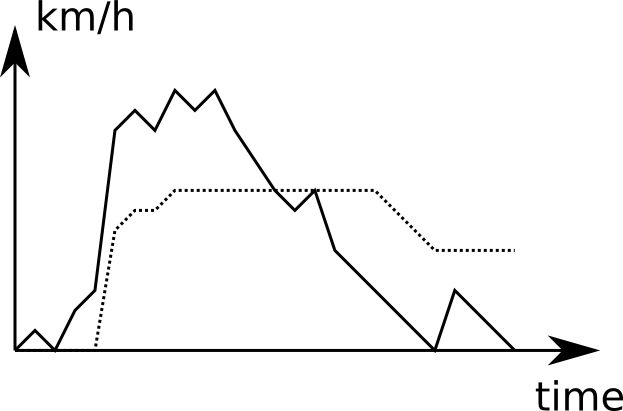
\includegraphics[width=0.4\textwidth]{../images/acckm.png}
\caption{Acckm}
\label{fig:acckm}
\end{figure}

\begin{figure}
\centering
\includegraphics[width=0.5\textwidth]{../src/images/acckmTrips.png}
\caption{Acceleration kilometers}
\label{fig:acckmTrips}
\end{figure}

\subsection{Stop and go}
Stop and go behaviour is not fuel efficient as more fuel is consumed when accelerating that when driving at a constant speed.
It is therefore interesting to see if the number of times a vehicle stops and drives on is correlated with km/l.
We say a vehicle is stop when it decelerations below 10 km/h and that it drives again when it accelerates up above 15 km/h.

%TODO: Experiments

Figure~\ref{fig:stopngoTrips} shows the number of stop-and-goes of each trip normalised with the length of that trip versus the km/l of the trip.
The size of the plot indicates the amount of fuel used in the trip and the color signals what class it has been asigned to.
We see that the trips in the \fuelHigh class have few stop and goes and about half of the trips in the \fuelMedium class have more stop and goes.

\begin{figure}
\centering
\includegraphics[width=0.5\textwidth]{../src/images/stopngoTrips.png}
\caption{Number of stop and goes}
\label{fig:stopngoTrips}
\end{figure}

%\clearpage
\begin{table}
\begin{tabular}{|l|l|l|l|}\hline
Name & Data type & Source & Description\\\hline
\var{vehicleid} & integer & ID & Unique identifier for vehicles\\\hline
\var{timestamp} & timestamp & GPS & Date and time of the record\\\hline
\var{longitude} & float & GPS & Longitude coordinate of the vehicle\\\hline
\var{latitude} & float & GPS & Latitude coordinate of the vehicle\\\hline
\var{speed} & float & GPS & Driving speed in km/h\\\hline
\var{compas} & integer & GPS & Direction of the vehicle in degrees. North (0), east(90), south(180) and west(270)\\\hline
\var{satellites} & integer & GPS & Number of visible satellites\\\hline
\var{rpm} & integer & CANBus & The engines rounds per minute\\\hline
\var{kmcounter} & float & CANBus & Mileage record\\\hline
\var{temperature} & float & CANBus & Temperature of the engine in degrees Celsius\\\hline
\var{throttlepos} & float & CANBus & Position of the throttle. No data available\\\hline
\var{fuellevel} & float & CANBus & Fuel level in the tank where 100 is full tank.\\\hline
\var{totalconsumed} & float & CANBus & Total amount of fuel consumed by the vehicle in liters\\\hline
\var{actualconsumed} & float & CANBus & Instantaneous amount of fuel consumption in liters. Undependable\\\hline
\var{actual\_km\_l} & float & CANBus & Instantaneous km/l. Undependable\\\hline
\var{acceleration} & float & CANBus & Acceleration ???\\\hline %TODO: What is this
\var{make} & integer & Haulier &The make of the vehicle. No data available\\\hline
\var{model} & integer & Haulier &The model of the vehicle. No data available\\\hline
\var{capacity} & float & Haulier & Number of possible passengers. No data available\\\hline
\var{weight} & float & Haulier & The weight of the vehicle. No data available\\\hline
\var{seqmentkey} & int & Map-matching & Seqment id for which seqment the vehicles was on\\\hline
\var{direction} & text & Map-matching & Either \var{FORWARD} or \var{BACKWARD} on the seqment.\\\hline
\end{tabular}
\caption{GPS and CANBus data types}\label{tb:dataDescription}
\end{table}
\clearpage
%%%%%%%%%% DO NOT EDIT ABOVE, THIS WILL BE AUTO GENERATED %%%%%%%%%%

% BIBLIOGRAPHY 
\bibliographystyle{abbrv}
%\bibliographystyle{plainnat}

%A void complaints from bibtex about no citations!
\raggedright % Disable justified right margin 
\bibliography{bibliography} %Put in a bibliography

% Appendix
%\justifying
%\clearpage
%\appendix
%\input{src/Appendix.tex}

\end{document}
